\large{
L'intero lavoro svolto si basa su due importanti settori informatici quali la teoria dei grafi e la visualizzazione delle informazioni. Queste due aree di studio saranno viste di seguito nel dettaglio.
\section{Visualizzazione delle informazioni}
La visualizzazione delle informazioni può essere definita come l'utilizzo o comunque l'impiego di rappresentazioni visuali ed interattive di dati astratti, con il compito di amplificarne la conoscenza degli stessi o anche come la comunicazione di dati attraverso l'utilizzo di interfacce visuali. Questo particolare settore è di grande rilievo sia per l'analisi dei dati che per la presentazione e quindi per la comunicazione degli stessi. Importante però è non assegnare alla visualizzazione delle informazioni il mero scopo di creazione di grafici privi di informazione in quanto essa è la base su cui si andrà a lavorare. \\
Per quanto riguarda i dati astratti citati prima, essi possono essere di due tipi, strutturati e non strutturati. I dati \textbf{strutturati} sono rigidamente formattati, si stima che siano soltato il 20\% dei dati che si producono e sono solitamente organizzati in tabelle. Quelli \textbf{non strutturati} risultano essere invece difficili da analizzare tanto che uno dei primi compiti antecedente la visualizzazione è quello di riuscire a trasformare dati non strutturati in dati tabellari o dati flat.
Per la rappresentazione dei dati inoltre sono di notevole importanza i principi di questo ambito informatico che prevedono le seguenti operazioni che precedono la visualizzazione dei dati:
\begin{itemize}
	\item\textbf{Estrazione:} download,caricamento o conversione dei formati;
	\item\textbf{Semplificazione:} operazioni di filtraggio rimozione e aggregazione;
	\item\textbf{Aggiustamento: } può riguardare operazioni matematiche e variazioni sul tipo di dato.
\end{itemize}
Definita la visualizzazione delle informazioni è necessario, evidenziare i principi per una rappresentazione dei dati corretta e soprattutto il modello di progettazione.
\textbf{Tamara Macushla Munzner} propone un modello per la visualizzazione orientato al task model composto da 4 fasi:
\begin{itemize}
	\item \textbf{Dominio:} identificazione del problema e del dominio di interesse;
	\item \textbf{Astrazione dei dati:} si modellano i dati che dovranno essere rappresentati;
	\item \textbf{idioma di codifica:} si decide come visualizzare i dati e quali interazione implementare all'interfaccia;
	\item \textbf{Algoritmo}.
\end{itemize}

Tra tutti questi principi del modello di Munzner inoltre esiste un rapporto di inclusione in cui dalla fase più esterna ad una più interna esiste un rapporto di molteplicità.
In altre parole a puro titolo di esempio diversi idiomi possono corrispondere alla stessa astrazione e diverse astrazioni possono corrispondere allo stesso dominio.\\
Esistono due tipologie di approccio per una visualizzazione orientata al task model. Il primo è quello dell'approccio \textbf{Top-Down}, ovvero guidato dal problema e risolto dal dominio fino all'algoritmo applicando le varie scelte progettuali. Il secondo è invece quello dell'approccio \textbf{Bottom-up} ed è guidato dalla tecnica.
Per concludere la digressione sui principi della visualizzazione è importante anche definire il concetto di \textbf{User-Task} come scopo dell'utente ovvero cosa deve poter fare sui dati.
Nella visualizzazione delle informazioni ci sono due principali tipi di scopi:
\begin{itemize}
	\item \textbf{Presentazione}, contesto in cui si conosce l'informazione e la visualizzazione è tesa a rappresentarla;
	\item \textbf{Analisi}, contesto in cui la visualizzazione è tesa all'estrazione delle informazioni dei dati rappresentati.
\end{itemize}

\section{Interazione}
Definendo la disciplina della visualizzazione delle informazioni come il mezzo per poter creare interfacce interattive per riuscire ad estrarre informazione dai dati  è necessaria adesso una digressione sul concetto di interazione dell'utente e delle sue primitive.
L'interazione assume definizioni diverse ma non discordanti tra loro a seconda dell'ambito di lavoro e del campo a cui questa fa parte. 
Per quanto concerne il campo della ricerca \textbf{HCI}, ovvero della Human Computer Interaction, l'interazione è stata definita già nel 1998 come la comunicazione tra uomo e macchina.
Per definire a pieno lo human-computer interaction e l'usabilità bisogna far riferimento al modello di Donald Arthur\textbf{ Norman}, psicologo e ingegnere statunitense. Egli identifica l'interazione utente-calcolatore nelle 7 fasi riportate di seguito: 
\begin{enumerate}
	\item formulare l'obiettivo
	\item formulare l'intenzione
	\item identificare l'azione
	\item eseguire l'azione
	\item percepire lo stato del sistema
	\item interpretare lo stato del sistema
	\item valutare il risultato rispetto all'obiettivo
\end{enumerate}
%%citare libro La caffettiera del masochista. Psicopatologia degli oggetti quotidiani (The psychology of everyday things e The design of everyday things,1988), Milano, Giunti, 1990 (ISBN 978-88-09-20182-8), 1997 (ISBN 978-88-09-21027-1), 2005 (ISBN 978-88-09-04419-7), 2009 (ISBN 978-88-09-74356-4).
Secondo \textbf{Norman} inoltre un principio fondamentale è capire gli utenti e i compiti che intendono svolgere facendo anche in modo che le interfacce utente consentano tali compiti nel modo più immediato e intuitivo possibile. Norman infine fa notare, nel suo libro "La caffettiera del masochista", come questo principio sia spesso inutilizzato.\\
Nel campo della ricerca nella visualizzazione delle informazioni all'interazione furono date più definizioni, una successiva temporalmente alle altre. Di seguito ne sono riportate due fondamentali:
\begin{itemize}
	\item \textbf{2002}: l’interazione consente la manipolazione diretta della rappresentazione grafica del dato;
	\item \textbf{2007}: l’interazione fornisce agli utenti la capacità di manipolare direttamente o indirettamente e modificare le rappresentazioni.
\end{itemize}
Già da queste definizioni è possibile notare la fondamentale importanza dell'interazione dell'utente poiché una rappresentazione senza la possibilità di modifica, restando comunque utile all'utente finale, potrà solo essere analizzata staticamente in quel suo ambito di verità. Grazie all'interazione l'utente non solo potrà eseguire task di analisi ma anche di manipolazione creando a sua volta nuove modalità di analisi ed acquisendo consapevolezza della fondamentale importanza del fattore umano sulla macchina.\\
Date le varie definizioni dell'interazione e definito il suo impiego nella visualizzazione delle informazioni è facile notare come tutte le interazioni dipendono da vari fattori che ne influenzano il comportamento e spesso anche il successo oppure il declino di una particolare modalità di visualizzazione.
Ogni interazione può inoltre essere classificata a seconda di vari fattori che sono introdotti di seguito:
\begin{itemize}
	\item \textbf{Tempo di risposta}:l'ordine di tempo a cui appartiene il tempo di risposta dell'interazione al comando dell'utente al sistema è la prima grande classificazione. Se il tempo di risposta risulta essere dell'ordine  dei $10^-1$ secondi l’interazione è velocissima e fa uso di animazioni e l'utente potrà eseguite tante operazioni in un tempo irrisorio, se risulta dell'ordine dei $10^0$ secondi l'animazione farà uso di dialoghi o finestre di dialogo che molto spesso indirizzeranno l'utente per future interazioni e se infine sarà superiore ai $10^1$ secondi interazioni saranno cognitive ovvero task che verranno eseguiti prima di ottenere risposte.
	\item \textbf{Azioni atomiche}: rispondono alla domanda "in che modo si eseguiranno le interazioni". Queste potrebbero essere eseguibili tramite tasti o azioni eseguiti con l'ausilio di un mouse o ancora potrebbero essere azioni di più alto livello come vocali, gestuali o touch.
	\item \textbf{Tecnologia}: una interazione non è nulla senza il dispositivo su cui la si esegue. Ricordando che differenti tipologie di dispositivi forniscono diversi tipi di interazioni si può classificare l'interazione anche mediante la scelta del dispositivo utilizzato che sia esso un laptops, un tablets o uno smartphone fino ad arrivare ad avere interazioni specifiche per dispositivi indossabili che riconoscono ad esempio i movimenti gestuali.
	\item \textbf{Grado di interazione}: ogni interazione possiede un grado definito come il livello di connessione e di padronanza delle operazioni che l'utente può ottenere interagendo con il sistema. In particolare il grado di interazione può essere:
	\begin{enumerate}
		\item \textbf{statico} ovvero grado $1$ in cui non è prevista alcun genere di interazione riducendo la rappresentazione ad una singola vista per una analisi non modificabile;
		\item \textbf{manipolabile} ovvero di grado $2$ in cui è possibile cambiare la vista della scena e quindi evidenziare ed analizzare meglio un dato dalla sua rappresentazione non potendo però modificare i dati da cui è nata la visualizzazione;
		\item \textbf{trasformabile} ovvero di grado $3$ dove l’interazione permette di intervenire nella fase di processo e cambiare il dato di input.
	\end{enumerate}
	\item \textbf{paradigma}: intesa come tipologia di interazione vera e propria che potrà essere tradizionale dove c’è un punto di comunicazione tra l’uomo e la macchina, realtà aumentata o la realtà virtuale.
\end{itemize}
Date le definizioni inserenti l'ambito della visualizzazione delle informazioni, si passa ora alle definizioni inerenti la teoria dei grafi.
\section{Grafi}

\begin{figure}[!htb]
	\begin{center}
		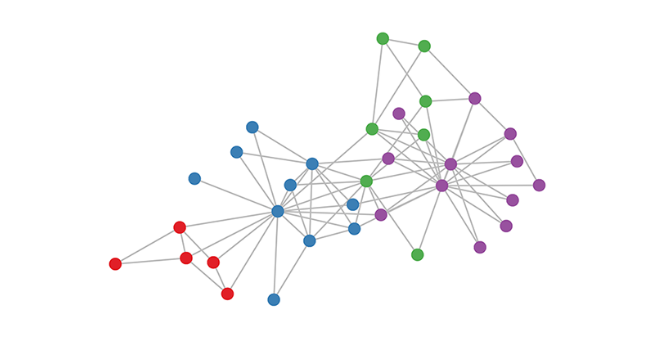
\includegraphics[width=0.7 \linewidth]{figure/grafoGenerico}
	\end{center}
	\caption{Esempio di grafo indiretto connesso \label{fig:grafoGenerico}}
\end{figure}
La teoria dei grafi è la disciplina che si occupa dello studio dei grafi, oggetti discreti che permettono di schematizzare una grande varietà di situazioni, processi e spesso di consentire delle analisi in termini quantitativi ed algoritmici. 
Un grafo G è definito da una coppia di insiemi \textbf{$<V,E>$} in cui V è un insieme di nodi o vertici che possono essere connessi tra loro mediante l'insieme di archi E tale che i suoi elementi siano coppie di elementi dell'insieme V esprimibile come
 $$E \subseteq V * V$$ 
Si definisce poi grafo \textbf{completo} un grafo in cui ogni vertice è collegato con tutti gli altri vertici rimanenti, di modo che l'insieme degli archi $E$ è esplimibile come $E= V * V$.
Dato un grafo è possibile avere un disegno $\tau(G)$ come mapping dei vertici su punti distinti del piano.\\
Si distinguono due tipi di grafi:
\begin{itemize}
	\item \textbf{non orientati}, dove la relazione $E$ è simmetrica, quindi $$(a,b) \in E \Rightarrow (b,a) \in E$$. In questo tipo di grafo, gli archi sono solitamente denominati spigoli e i nodi vertici.
	\item \textbf{orientati}, dove la relazione E non è simmetrica ed esiste una relazione d'ordine tra i nodi.
\end{itemize}
In un grafo infine si definisce ciclo (o circuito) di lunghezza $m$ una catena $(v0, ..., vm-1, v0)$.
Si dice inoltre ciclo semplice un ciclo che non passa due volte dallo stesso nodo, o formalmente un ciclo $(v0, ..., vm-1, v0)$ per il quale:
$$\forall i,k=1,...,m-1,(i\neq k\Rightarrow v_{i}\neq v_{k})$$

I grafi risultano comunque essere una delle strutture fondamentali su cui si basano molte applicazioni reali ed anche il principio fondamentale alla base del lavoro svolto.

\section{Alberi} 
Data la definizione di grafo, si può definire un albero \textbf{tree} come un grafo connesso non orientato e senza cicli come mostrato in \textbf{\figurename~\ref{fig:alberoGenerico}}.\\
Per essere tale quindi il grafo in questione deve possedere un solo cammino per ogni coppia di vertici oppure essere aciclico massimale.
Ogni nodo appartenente ad un albero possiede un livello dato alla somma $ 1 + l(padre) $ intendendo che la radice dell'albero ha livello 0.
\begin{figure}[!htb]
	\begin{center}
		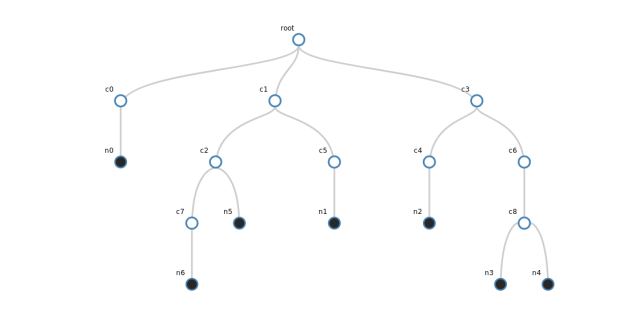
\includegraphics[width=0.8 \linewidth]{figure/alberoGenerico}
	\end{center}
	\caption{esempio di albero n-ario \label{fig:alberoGenerico}}
\end{figure}
La radice è definita come l'unico nodo dell'albero che non possiede archi entranti ma solo archi uscenti e a cui solitamente viene data rappresentazione del livello più basso dell'albero in altre parole è l'unico nodo che non presenta nodi con livello inferiore(i nodi padri) ma solo nodi con livello superiore(i nodi figli). 
Per completezza si voglio dare anche le definizioni di profondità di un nodo e di altezza di un albero rispettivamente come la lunghezza del cammino dalla radice al nodo e la profondità massima dei suoi nodi.
I nodi dell'albero diversi dalla radice possono inoltre essere partizionati in due categorie:
\begin{itemize}
	\item\textbf{nodi interni}: definiti come nodi con almeno un figlio e suddivisibili ulteriormente in nodi bassi, in cui tutti i figli sono foglie ed in nodi alti, che possiedono almeno un nodo interno come figlio;
	\item\textbf{foglie }che non possiedono figli e per questo non hanno archi uscenti.
\end{itemize}

\begin{figure}[!htb]
	\begin{center}
		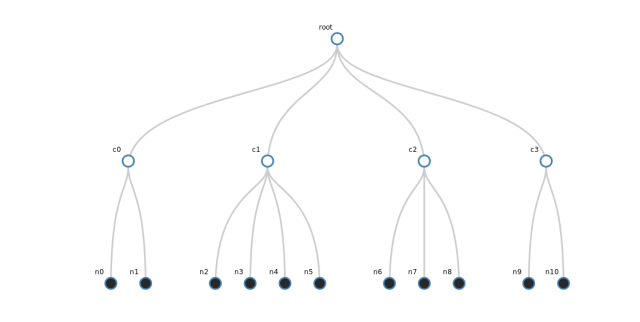
\includegraphics[width=0.8 \linewidth]{figure/flatTree}
	\end{center}
	\caption{esempio di flat Tree \label{fig:flatTree}}
\end{figure}
Un nodo è inoltre definibile \textbf{omogeneo} se tutti i suoi figli sono foglie oppure tutti nodi interni.
Data la definizione di nodo omogeneo, viene detto che un albero è omogeneo se e solo se tutti i suoi nodi sono nodi omogenei.
Si definisce poi $S(T)$ come la dimensione dell'albero $T$, ovvero il numero di nodi superiori di $T$ diversi dalla radice.
Date queste definizioni introduttive relative agli alberi è possibile definire un albero flat (come mostrato in \textbf{\figurename~\ref{fig:flatTree}}) con il lemma seguente:
\begin{center}
	\textit{Un albero omogeneo T di altezza $h(T)>= 2$ e dimensione $S(T)> 0$  e che contiene almeno un nodo $\mu^*\neq r(T)$ in modo tale che $T(\mu^*)$ è flat}
\end{center}
Definendo in questo modo un albero flat è facile notare come ogni albero flat è anche omogeneo, avendo tutti i nodi interni che hanno come figli esclusivamente foglie ed il nodo radice che possiede solo nodi interni.\\
}

